\documentclass[11pt,letter]{article}
\usepackage[top=0.50in, bottom=0.7in, left=1.1in, right=1.1in]{geometry}
\usepackage{graphicx} % Required for inserting images
\usepackage{xcolor} 
\definecolor{Accent}{HTML}{bd2b00} 
\usepackage[numbers,compress,super]{natbib}
\usepackage{gensymb}
\usepackage{hyperref}
\hypersetup{colorlinks,citecolor = Accent, linkcolor = Accent,urlcolor = Accent, breaklinks=true}
\usepackage{cleveref}
\usepackage[labelfont=bf]{caption}
\bibliographystyle{unsrtnat}

\RequirePackage[labelfont={bf,sf},%
                font={small, sf}]{caption}

\usepackage{lineno}
\renewcommand\linenumberfont{\normalfont\tiny\color{gray}}

\begin{document}

\title{Overlooked model uncertainties may misinform forest management strategies}

\author{Victor, Jérôme, Isabelle, and more?}
\date{}
\maketitle 


\noindent\rule{\textwidth}{0.3pt}
\textbf{Abstract:} Forests play a major role in mitigating climate change, but increasing threats to forests from climate change have heightened the importance of managing these systems. Robust forecasts of forest composition with increasing climate change are critical to this aim, but are currently highly variable. To help guide management in the face of this variability and understand where we can most rapidly reduce uncertainty through improved models, we compare over XX ecological models and climate scenarios in forecasts for forests across Europe. Our approach considers a gradient of more mechanistic (`process-based') to correlative models of species distributions to find that uncertainty in ecological models can drive more variation than vastly different climate scenarios (e.g., SSP2 vs. SSP5), but also areas with relatively consistent projections [give overview of these and say that this could reduce uncertainty in how to manage for these areas]. [Maybe something on using existing range data leads to more pessimistic forecasts?] Our results highlight a new way to approach ecological forecasting that better identifies areas of higher certainty and, conversely, the areas where managers will need more diversified approaches and where more ecological study may be most useful. % pick: significant local variation OR diverse trade-offs

\noindent\rule{\textwidth}{0.3pt}

\linenumbers

\subsection*{Main}
%
%Intro:
%1. Basically first two paragraphs you have combined (we need forests to
%store C, and they are doing poorly) ending on the need for better
%guidance of forest management
%2. This is hard because we have a lot of biological models and they give
%different answers, and for management we need to layer on the future
%climate models ...
%- Go into briefly the correlative versus process models -- they
%differ  but we're not sure which is best
%- Given we don't have one great approach to build to (and we have
%run out of time), so maybe we move on and accept the diversity
%- Transition to something explaining the layers of models we need
%to consider to capture climate to biology
%3. Back to what we need to do with the models for forest management
%- Here you might touch on what we could do with this, get in some
%of the stuff I highlighted in the discussion that you need to foreshadow
%for readers.


%From J Chave:
%Climate change has direct impact on a myriad of ecosystem processes, and forests are especially vulnerable. European temperatures are rising twice as fast as the global average (Copernicus Climate Change Service, 2024), and unprecedented pulses of tree mortality have benn reported in the last decade, across the range of forest species (Senf et al, 2020). As a consequence, some European forests are now net CO2 sources (Hadden and Grelle, 2016; Karelin et al, 2021), due to decreased growth (Hadden and Grelle, 2016; van der Woude et al, 2023), increased burned areas (Carnicer et al, 2022; Kelly et al, 2024), and increased pest or drought-related dieback driven (Cienciala and Melichar, 2024; Karelin et al, 2021; Latifovic and Arain, 2024).  Implementation strategies are rolled out in spite of the uncertainty of the scenarios.

%1. Basically first two paragraphs you have combined (we need forests to
%store C, and they are doing poorly) ending on the need for better
%guidance of forest management
% the baby: with climate change, we need to safeguard and adapt forests, as they play a major role in mitigating its effects
Forests are key to pursuing climate change mitigation policies and achieving carbon neutrality  \citep{Korosuo2023, Hyyrynen2023}. Yet, forests are increasingly under pressure. In Europe, temperatures are rising twice as fast as the global average \citep{CCCS2024}, and unprecedented pulses of tree mortality  have been reported in the last decade \citep{Senf2020}. As a result, some European forests are becoming net CO$_2$ sources \citep{Hadden2016, Karelin2021}, due to decreased growth \citep{Hadden2016, Woude2023}, larger burned areas \citep{Carnicer2022, Kelly2024}, and increased pest- and drought-induced dieback \citep{Karelin2021, Cienciala2024, Latifovic2024}. Forest managers are facing unprecedented challenges, as they must address current threats while also promoting long-term adaptation to climate change. In this context of high uncertainty, better guidance is needed to implement successful strategies.


%2. This is hard because we have a lot of biological models and they give
%different answers, and for management we need to layer on the future
%climate models ...
%- Go into briefly the correlative versus process models -- they
%differ  but we're not sure which is best
%- Given we don't have one great approach to build to (and we have
%run out of time), so maybe we move on and accept the diversity
%- Transition to something explaining the layers of models we need
% the werewolf: We have many models, we don't know which one is the best. Most decisions rely on limited models without much insight into what drives differences in projections. This can mask significant uncertainties and ultimately threaten the success of forest management decisions
% the silver bullet: accept a greater diversity of models (scientific approaches, hypothesis), and figure out how to safeguard forests by gaining a better understanding of uncertainties, i.e., merging across biological and climatological components (uncertainty budget framework)
Given the diversity of predictive ecological models, the challenge of providing practical insights for forest management is even greater. Different models, ranging from correlative to more mechanistic approaches, may provide highly divergent projections \citep{Morin2009, Keenan2011a, Cheaib2012, Takolander2019}. While it remains unclear under which conditions one approach is more reliable than another \citep{VanderMeersch2024}, most forecasting studies still rely on a limited set of models \citep{Dyderski2018, Wessely2024, Hanewinkel2013, Schueler2014}. We thus often lack a comprehensive understanding of what drives differences between projections \citep{Simmonds2024}. Given the urgency of climate change, we must incorporate this diversity and merge across ecological and climatological models to provide a complete picture of both the threats and opportunities for forests. 

%3. Back to what we need to do with the models for forest management
%- Here you might touch on what we could do with this, get in some
%of the stuff I highlighted in the discussion that you need to foreshadow
%for readers.
Gaining a better understanding of where uncertainties originate and how they relate is crucial to identify opportunities 
% for model developments \citep{Petchey2015} and  % maybe off-topic? keep for discussion?
to address policy-relevant questions \citep{Urban2016}. Species shifts are predicted to have major impacts on timber production and on the forest economic sector \citep{Wessely2024, Hanewinkel2013}. Forest managers need to know whether the current species will be able to tolerate future climate conditions, whether they can rely on its natural regeneration, or whether they should capitalize on new species opportunities. If the main driver of variation across projections is the different ecological models, even more than different global emissions scenarios, it becomes critical to encompass the full range of models. Failing to do so could lead to overly confident predictions about which species will or will not be able to survive in future climates, ultimately leading to counterproductive or even detrimental forest management decisions.

To understand the level of confidence we can place in predictions requires a framework that account for all the various components of climatological and biological uncertainties, including socio-economic scenarios, global climate models, ecological models, down to the species level. To this aim, we combined over 1,500 projections of forest tree species distributions, incorporating a wide range of models, from more mechanistic (‘process-based’) to correlative models. Fully accounting for our current level of knowledge about future climate states and species functioning allows us to quantify the contribution of each component to the total variation across projections. This approach represents a significant advancement over previous studies, which overlooked large portions of uncertainty, and will lead to better informed decision-making to improve the resilience of forests.

% Note: what should be in the intro:
% huge differences between projections, more importanmt than species or SSP, toget a comprehensive assesment of the magnitude of climatic change?
%  ignoring a large portion of uncertainty in psecies range projections due to modelling approaches can thus lead to baaad decisions.

\subsection*{Results and discussion}

Our dataset included 9 tree species, both deciduous and coniferous, adapted to diverse climatic conditions across Europe. We simulated their suitability from 1970 to 2100, at a 0.1\degree~spatial resolution, using a diverse set of ecological models spanning different hypotheses and calibration methods. For future projections, we used 10 different climate simulations, based on 2 forcing scenarios and 5 global climate models with different climate sensitivities.

% uncertainty in ecological models can drive more variation than vastly different climate scenarios 
Across species, ecological models drive more variation than vastly different climate scenarios. They consistently represent the major source of uncertainty across major European biomes (explaining between 42.9\% and 63.9\% of the variation between projections), with the exception of the Alpine biome. At the species-level, the differences between ecological models is also the main source of uncertainty for all the species considered here, and represents between 40\% and 62\% of the total uncertainty on average. One of the striking example is the climatic suitability change of sessile oak in the Atlantic region, where this species represents an important cultural and economic value, and for which more than 80\% of the uncertainty in climate change impact projections was due to variations among ecological models. 

% The differences among climate model projections (GCMs) and socioeconomic scenarios (SSPs). 
% in the Continental ecoregion, differences across models account for 73.7% of the total uncertainty of beech future suitability, despite being within the core of its present distribution. Similarly, SDM is the main source of uncertainty for sessile and pedunculate oaks (respectively 57% and 76.8%, Figure 22).

\begin{figure}
	\centering
	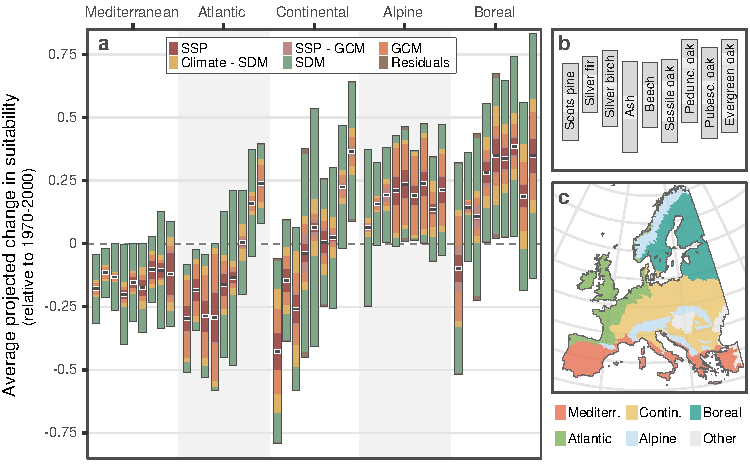
\includegraphics[width=0.7\linewidth]{../newfigures/files/figure1}
	\caption{}
	\label{fig:anovaspecies}
\end{figure}

Failing to account for a broad range of ecological models bias our level of confidence in them. Considering only correlative models would have misled to an overestimation of the contribution of climate projections (forcing scenarios, climate models, and their two-way interaction) to the total projection uncertainty in all regions, except the Mediterranean. In particular, divergence between climate models would have appeared to contribute as much as ecological models to projection uncertainty (on average, 36.6\% and 37.5\%, respectively). By accounting for more diverse ecological models, as done in our study, the uncertainty introduced by different ecological models (51.0\% on average) is greater than that introduced by climate models (19.9\% on average) for all the species. One of the key challenges for reducing uncertainty remains at the biological and ecological levels, even before considering the broad variations across future climate projections.
% At biome scale: e.g. continental: 54.3% of SDM with full diveristy (GCM: 14.10%), only 27.95% when considering only correlative models (46.22% for GCM)
% Also true a the species-level: SDM 50.77 down to 27.46, GCM 15.85 up to 35.95%

% For example, for beech, we would have estimated that discrepancies between GCMs would have been the major source of uncertainties (39.8\%), higher than the SDM uncertainty (33.8\%), whereas it was in reality much lower (18.8\%) than SDM uncertainty (51.2\%) when considering the three approaches of SDMs. Ignoring a large portion of uncertainty in species range projections due to modelling approaches can thus lead to overly confident predictions about which species will or will not be able to survive in future climates.  This becomes increasingly true as we approach the end of the 21\textsuperscript{st} century, where larger climate changes result in larger variation among projections (\Cref{fig:anovaecoregions}).
% there is a strong interest in considering a broader range of models to better characterize projections uncertainty.

\begin{figure}
	\centering
	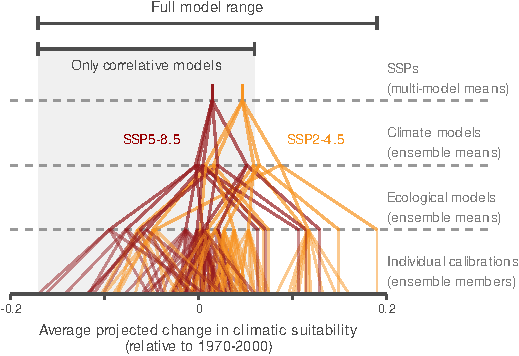
\includegraphics[width=0.7\linewidth]{../newfigures/files/uncertaintycascade}
	\caption{Temporary figure}
	\label{fig:manag}
\end{figure}

% [Maybe something on using existing range data leads to more pessimistic forecasts?]
Our results also revealed that the divergent projections between ecological models followed a regular pattern. Models (correlative or mechanistic) calibrated using current species range data consistently projected stronger decrease in climatic suitability for all species than models calibrated using other data (e.g. experimental). 
predict greater extinctions at the southern edge of species ranges
greater extinctions at the warmer limits (generally southern)
%Especially in Mediterranean and Atlantic ecoregions and in the western part of the Continental ecoregion (Figures 23). Overall, expert PEMs also simulated a higher increase of suitability in the transition zone between Continental and Boreal ecosystems. Fitted PEMs
%Taking a vue restrictive des modeles weakens the robustness of projections.
These discrepancies between models can significantly alter country-level projections, and impact national strategies derived from them. In Germany for example, beech showed an average suitability decrease of -0.04 ($\pm$0.09) in 2090 when considering only models entirely calibrated with current species distribution data, whereas...
Distribution data may not capture the full climatic niche of a species, underestimating the range of conditions where it could survive \citep{Chevalier2024, NoguesBravo2016}.
Relying on a narrow set of models---especially derived from the same calibration process (too technical?)---undermines the robustness of projections!


% \item which implications in terms  of forest management? 
%\begin{enumerate}
%	\item on average, uncertain projections = more possibilities to act? more adaptation measures
%	\item but high uncertainties may lead to \emph{laissez-faire}
%	\item we want to avoid that, how to translate uncertainties into decision-making?\\
%	$\rightarrow$ favor forest adaptation strategies resilient to a wide range of possible future conditions.
%	\item forest managers, policy makers:\\
%	rethink the way species distribution modeling is applied to forest management\\
%\end{enumerate}

Comparing diverse models enable to identify areas with relatively consistent projections that differ in terms of future climate risks and levers of action to address them.
Around the Mediterranean Basin, the models consistently predict less favorable climatic conditions for the species we considered here. In areas where most species are threatened, forest managers may consider introducing new species, more drought-tolerant. In the Atlantic margin, the suitability of most species is also projected to decrease, except for the two Mediterranean species (pubescent and evergreen oaks). In some areas, evergreen oak has already replaced beech \citep{Penuelas2003}. Mechanistic model projections are less pessimistic for deciduous oaks and beech in France, suggesting that some better-adapted populations could survive if the existing standing genetic variation is maintained and promoted by forest managers \citep{Brang2014}. An other lever of action, practices: reduce forest density.
Continental: exhibit less clear trends, notable low agreement among ecological models, as well as the mountainous regions at the transition between Mediterranean and Continental/Atlantic climates (Pyrenees, Massif Central, Balkans). 
% But all agree on a lower suitability for Pinus sylvestris (variation is more due to climatic models and scenarios, 45.7%, than to ecological models, 30.8%), which is a commercially very important species [cite] in several countries of Central Europe (Poland, Eastern Germany, Czech Republic, Belarus).
% Projections seem to show that temperate deciduous species (e.g. beech, deciduous oaks) will be less affected, despite high uncertainties, mostly driven by high divergence among ecological models (between 45.7 and 75.4%).
% -> diversifcation of species, favor mixed forests? and developp economic filiere pour especes decidues
% one of the strategies to consider is the diversification of tree species, but also an increased genetic diversity within populations, to mitigate the risks associated with uncertain future conditions \citep{Morin2014, Ammer2019, Pretzsch2021, Vospernik2024}
% Finally, where high risks and low confidence, diversification of forest management practices is also important, favor uneven-aged stands [cite]
Boreal biomes in Scandinavian and Baltic countries are projected to get an overall increase of climatic suitability. These are mostly dominated by two conifers species, favoured by commercial forest management
Thanks to a more favourable climate and an extended growing season, temperate deciduous species can become more competitive at the northern margin of their range \citep{Bolte2010}. Lever of action: convert pure coniferous stands into mixed forest in order to increase their resilience \citep{Schauer2023}
% In the Boreal ecoregion – where two very important forestry countries in terms of wood stock, added value, and forest-based workforce are located (Finland and Sweden) – SDM approaches are even a higher source of uncertainty (33.7% on average) than the difference across species (14.4%).
% Climatic suitability is also projected to increase in the Alps and in the Scandinavian Mountains, but these areas are subject to a greater uncertainty related to climate projections (Figure 20), likely due to the more complex topography.
% a strong interest in considering a broader range of models to better characterize projections uncertainty

%  [give overview of these and say that this could reduce uncertainty in how to manage for these areas]
% At the continental scale, it is possible to distinguish several regions 
% 
% In particular, the suitability of temperate broadleaf species (sessile and pedunculate oaks, beech) is projected to decrease while that of Mediterranean species (pubescent and evergreen oaks) is projected to increase. 

% , part of Poland and low mountain ranges of Central- Eastern Europe (Carpats, Ore Mountains, Sudetes)

% Boreal
% temperature and length of the growing season are the main climatic variables which determine forest productivity in the boreal climate zone.
% 


% Multi-model ensembles have been so far mostly restricted to statistical models (Simmonds et al, 2024), but we show here that there is a strong interest in considering a broader range of models to better characterize projections uncertainty. 
% Europe: 38.6% forest, and most countries have at least 30% of forest
% Germany account for 13.2% of the stock of timber in the EU's forests 
% Sweden: 12.6% - France : 11.8%, then Poland, Finland Romania, all > 8%
% => these five countries represent more than 50%
%  largest workforce: Sweden, Romania, Germany

% Continental
%Large zones of Europe though exhibit . There is a notable low agreement among models in the Continental ecoregion, which includes some countries with important forest sector (Germany, Romania...), as well as in the British Isles (except Scotland). 
%In Atlantic and Continental regions, the differences between species are strong: all models agree with a lower suitability for fir and a higher suitability for holm and pubescent oaks, two Mediterranean species (Figure 22).
%In those regions, species-related uncertainty plays a major role (\Cref{fig:anova2090A}) and indicates that . Such unclear trends are also visible.

%Beyond the differences between SDM approaches, multi-model projections are particularly useful for identifying general trends and guiding forest management. Such At the continental scale, it is possible to distinguish several regions that differ in terms of future climate risks and levers of action to address them (Figure 21). Around the Mediterranean Basin and in South-western France, the models agree in predicting generally less favorable climatic conditions for the species we considered here. . However, process-explicit model projections are more nuanced for deciduous oaks and beech in France, suggesting that some better-adapted populations will survive if the existing standing genetic variation is maintained and promoted by forest managers (Brang et al, 2014). On the contrary, the Scandinavian and Baltic countries, part of Poland and low mountain ranges of Central- Eastern Europe (Carpats, Ore Mountains, Sudetes) are projected to get an overall increase of climatic suitability. Thanks to a more favourable climate and an extended growing season, beech has been shown to be already more competitive at the northern margin of its range (Bolte et al, 2010), and could be favoured to convert pure coniferous stands into mixed forest in order to increase their resilience (Schauer et al, 2023). Climatic suitability is also projected to increase in the Alps and in the Scandinavian Mountains, but these areas are subject to a greater uncertainty related to climate projections (Figure 20), likely due to the more complex topography.
%Large zones of Europe though exhibit less clear trends. There is a notable low agreement among models in the Continental ecoregion, which includes some countries with important forest sector (Germany, Romania...), as well as in the British Isles (except Scotland). In those regions, species-related uncertainty plays a major role (\Cref{fig:anova2090A}) and indicates that one of the strategies to consider is the diversification of tree species, but also an increased genetic diversity within populations, to mitigate the risks associated with uncertain future conditions \citep{Morin2014, Ammer2019, Pretzsch2021, Vospernik2024}. Such unclear trends are also visible in the mountainous regions at the transition between Mediterranean and Continental/Atlantic climates (Pyrenees, Massif Central, Balkans). Finally, in some areas where most species are threatened, forest managers may consider introducing new species, more drought-tolerant. 

\begin{figure}
	\centering
	\includegraphics[width=1\linewidth]{../newfigures/files/figure4}
	\caption{Temporary figure}
	\label{fig:manag}
\end{figure}

Looking ahead: a call to action for the scientific community...
%\begin{enumerate}
%	\item substantial progress required to develop more reliable projections
%	\item proper evaluation of the transferability?
%  	\item far from l'opposisiton non constructive de differentes ecoles, hypotheses, bridge across to gain practical insights
% Model refinement should rely not only on sophistication (i.e. adding new processes and parameters), but also on a step-by-step reassessment and reformulation of the model assumptions, take advantage of interdisciplinary synergies to build models that are not only grounded in the current scientific understanding of the processes but also statistically robust
%	we have to learn from the different approach, integrate them, of fewer, but more robust models that incorporate mechanistic understanding? simple models can also be great, especially at this scale! considering more diverse data, e.g. phylogeny
% statistical models are evolving towards more mechanistic approaches, recent trend to refine correlative models relies on the integration of more precise data (e.g. measured physiological parameters, \citealp{Kuo2022})
%	\item going further into uncertainty evaluation? (parameter uncertainty is totally ignored in process-explicit models...), robust inference methods to improve uncertainty propagation
%	$\rightarrow$ us, as scientists, we need to expose these uncertainties if we want forest managers to tackle them (transparency), i.e; we need to build on similar framework to actually guide adaptation
%\end{enumerate}


\clearpage

\bibliography{phd_bibliography}

\end{document}
